\chapter{Methods}
\section{Semantic segmentation}
\subsection{DeepLab}
One of the challenges in semantic segmentation using standard CNNs is that as the input feature map goes through the network
it gets smaller and the information about objects of a smaller scale can be lost.
DeepLab family introduces atrous convolutions that extract more dense features
which help to preserve the object's information. Compared to standard convolutions, atrous convolutions have an additional parameter, atrous
rate, which is the stride at which the input is sampled (Figure~\ref*{fig:aconv} a).
The atrous convolution is used in the last few blocks on features that were extracted from the backbone network (e.g. ResNet~\cite{he2016deep}).

\begin{wrapfigure}{r}{0.5\textwidth}
  \centering
  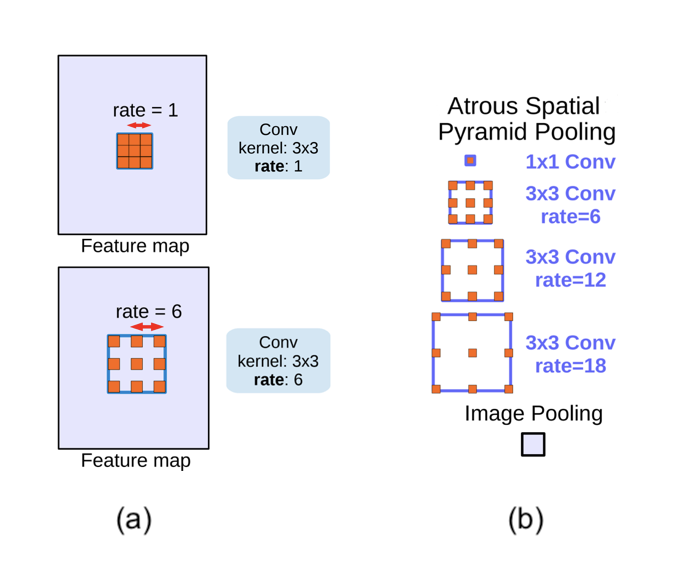
\includegraphics[width=0.5\textwidth]{figures/conv_aspp.png} %choose your uploaded image from folder "Images"
  \caption{(a) Atrous convolution, (b) ASPP augmented with Image Pooling (or Image-level features) ~\cite{chen2017rethinking}} %figure caption
  \label{fig:aconv} %labelling for internal reference
\end{wrapfigure}
One of the latest models in this family, DeepLabv3~\cite{chen2017rethinking}, applies several parallel atrous convolutions with different atrous rates
(Atrous Spatial Pyramid Pooling, or ASPP, Figure~\ref*{fig:aconv} b) to effectively capture multi-scale information. 
Image-level features, or image pooling, are also applied to incorporate global context information. Those are calculated by applying global average pooling on the last feature map of the backbone.
After applying all the operations in parallel, the results of each operation along the channel is concatenated and 1$\times$1 convolution is applied to get the output.
The addition of atrous convolutions allows the enlargement of the field of view without
increasing the size of the filtering kernel, therefore no increase in the computation time.
\subsubsection{DeepLabv3+}
The reproduction of shape contours during semantic image segmentation remained difficult with DeepLabv3~\cite{chen2018encoder}.
DeepLabv3 bilinearly upsamples the logits both during training and evaluation (Fig.~\ref*{fig:deeplab} a), hence
the improvements were made to employ the encoder-decoder structure (Figure~\ref*{fig:deeplab}) to avoid using a naive decoder.
\begin{figure}[h] %h=here; t=top; b=bottom of the page
  \centering
  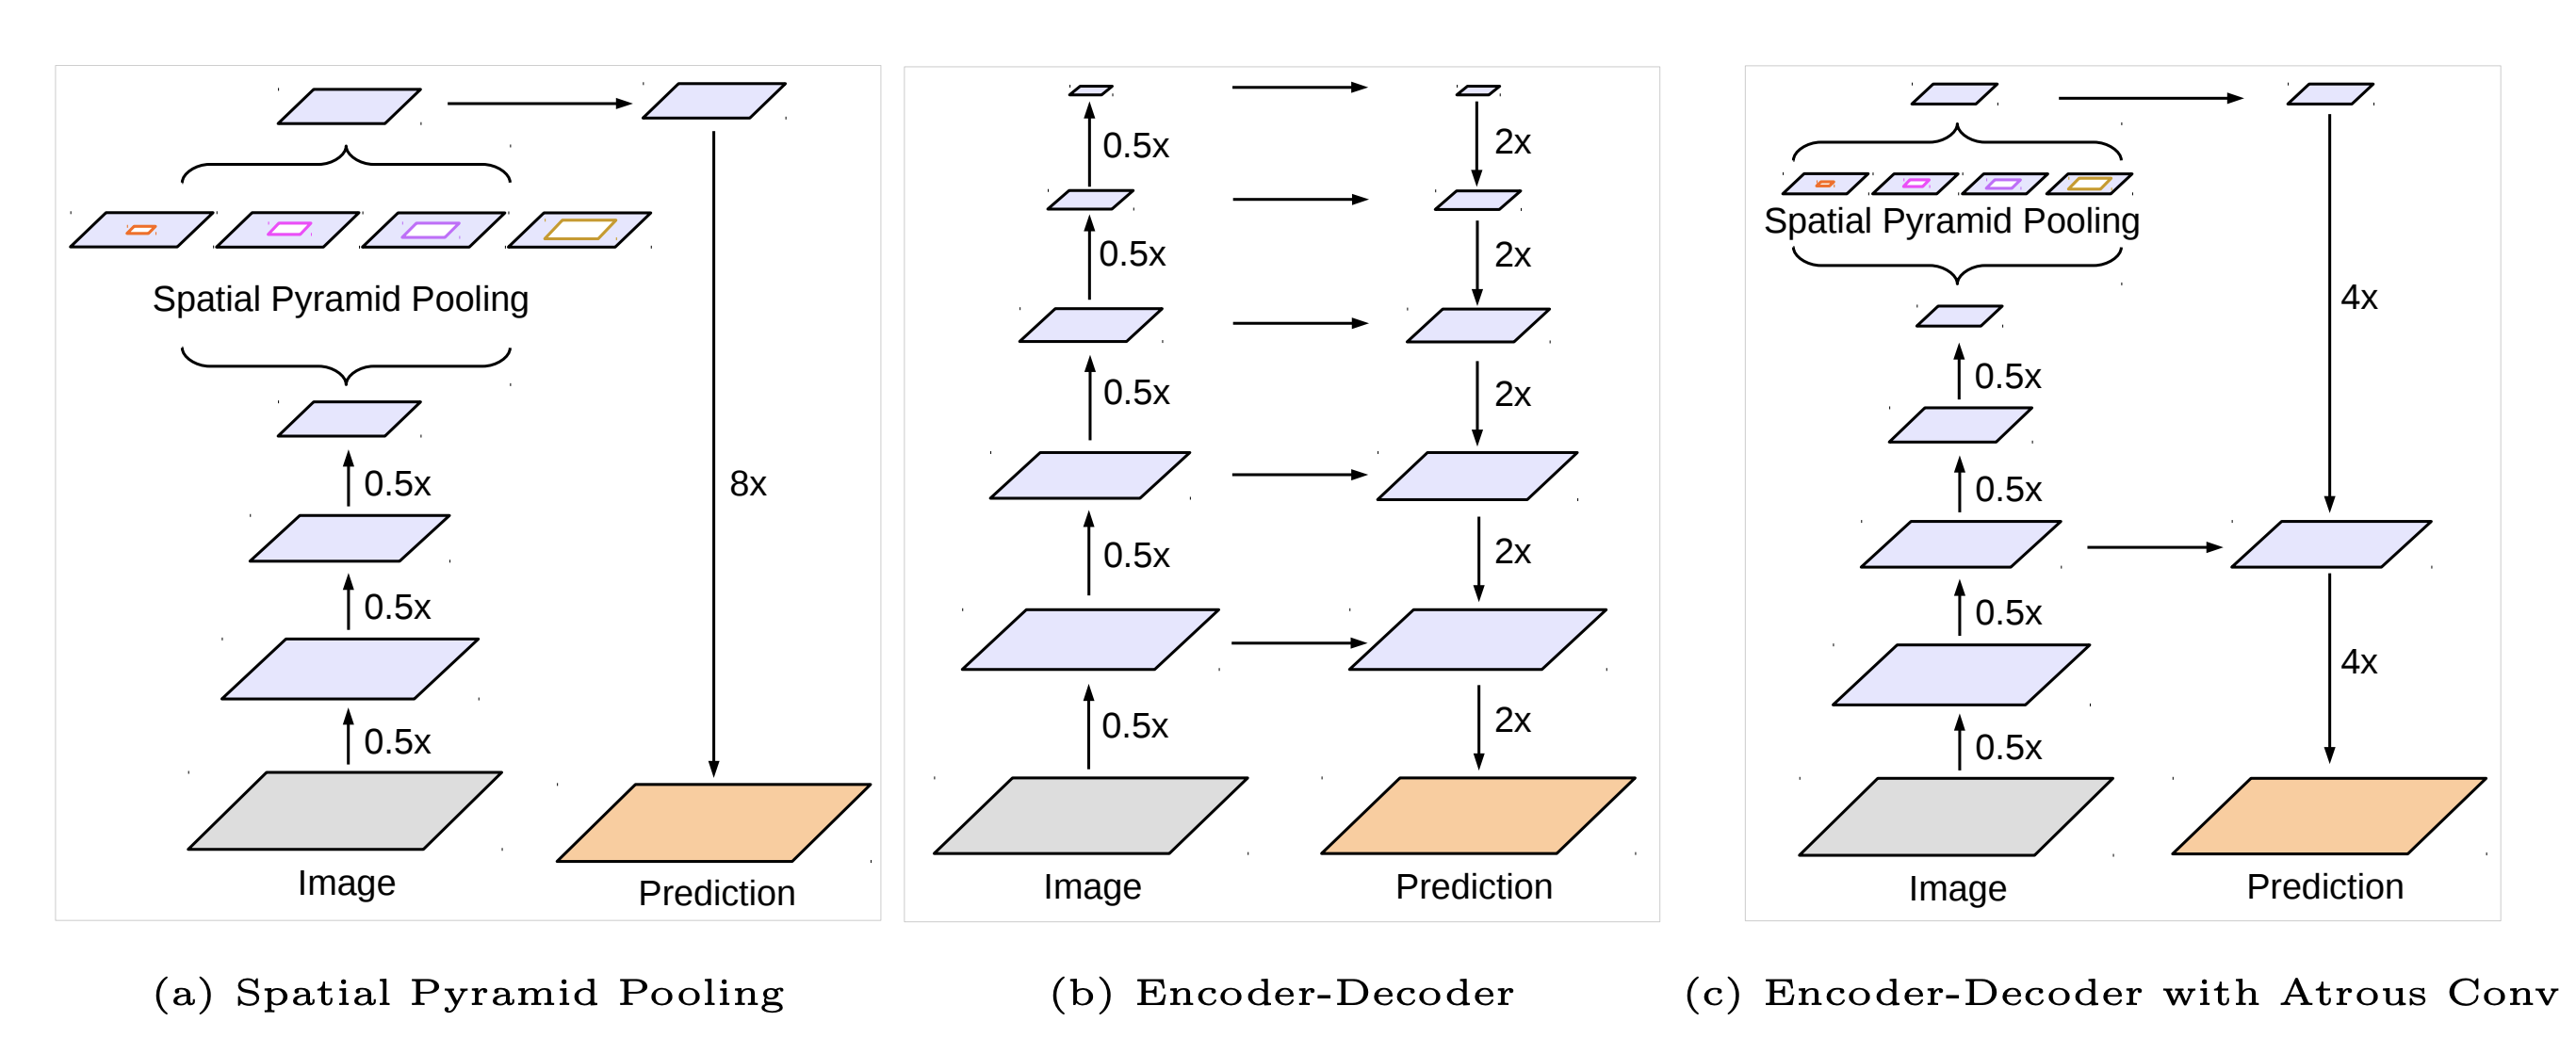
\includegraphics[width=0.9\textwidth]{figures/deeplab_encoderdecoder.png} %choose your uploaded image from folder "Images"
  \caption{The spatial pyramid pooling module of DeepLabv3 (a), the encoder-decoder structure (b) and DeepLabv3+ adaptation (c) \cite{chen2018encoder}} %figure caption
  \label{fig:deeplab} %labelling for internal reference
\end{figure} 
DeepLabv3+~\cite{chen2018encoder} adds the decoder module on top of the encoder output, as shown in Fig.~\ref*{fig:deeplabv3plus}.
In the decoder module, the 1$\times$1 convolution reduces the channels of the
low-level feature map from the encoder module which is then concatenated with the
DeepLabv3 feature map and the 3$\times$3 convolution obtains sharper segmentation results.
As a result, DeepLabv3+ holds rich semantic information from the encoder module,
while the detailed object boundaries are recovered by the decoder module and the spatial information is retrieved.
\begin{figure}[h] %h=here; t=top; b=bottom of the page
  \centering
  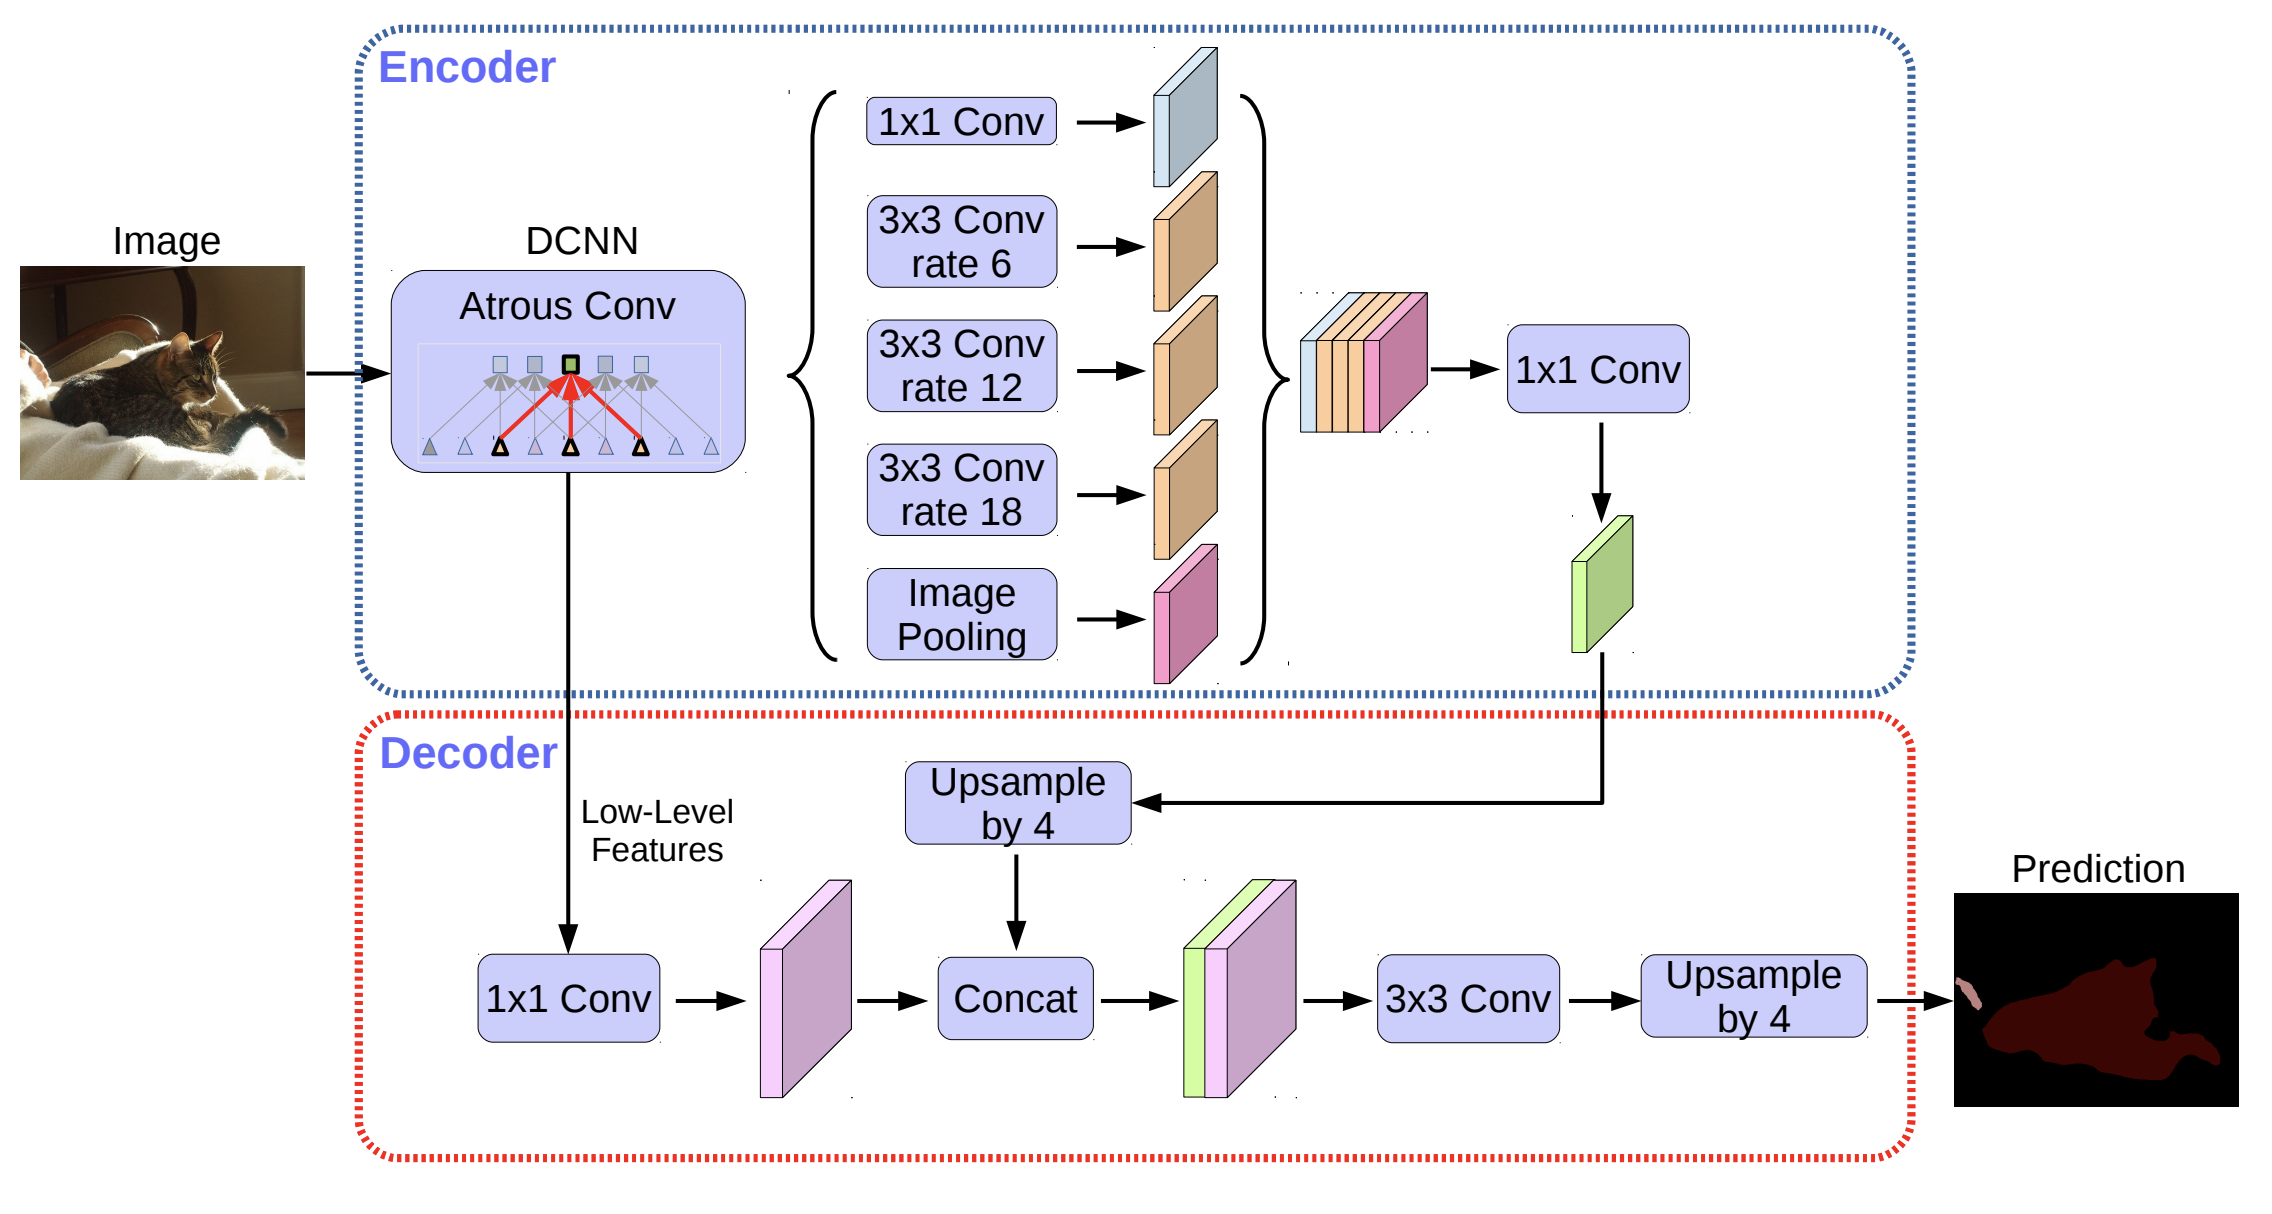
\includegraphics[width=0.9\textwidth]{figures/deeplabv3plus.png} %choose your uploaded image from folder "Images"
  \caption{DeepLabv3+ architecture. DeepLabv3 as encoder and proposed decoder structure for semantic image segmentation. \cite{chen2018encoder}} %figure caption
  \label{fig:deeplabv3plus} %labelling for internal reference
\end{figure} 

\subsection{Transformers}
\label{trans}
Transformers~\cite{vaswani2017attention} were originally designed for the neural machine translation problem in NLP to capture long-range dependencies among words in a sentence.
Their architecture converts one sequence into another one based on encoder-decoder architecture,
but it differs from the previously existing sequence-to-sequence models because
it does not imply any Recurrent Networks. 
\begin{wrapfigure}{r}{0.45\textwidth}
  \centering
  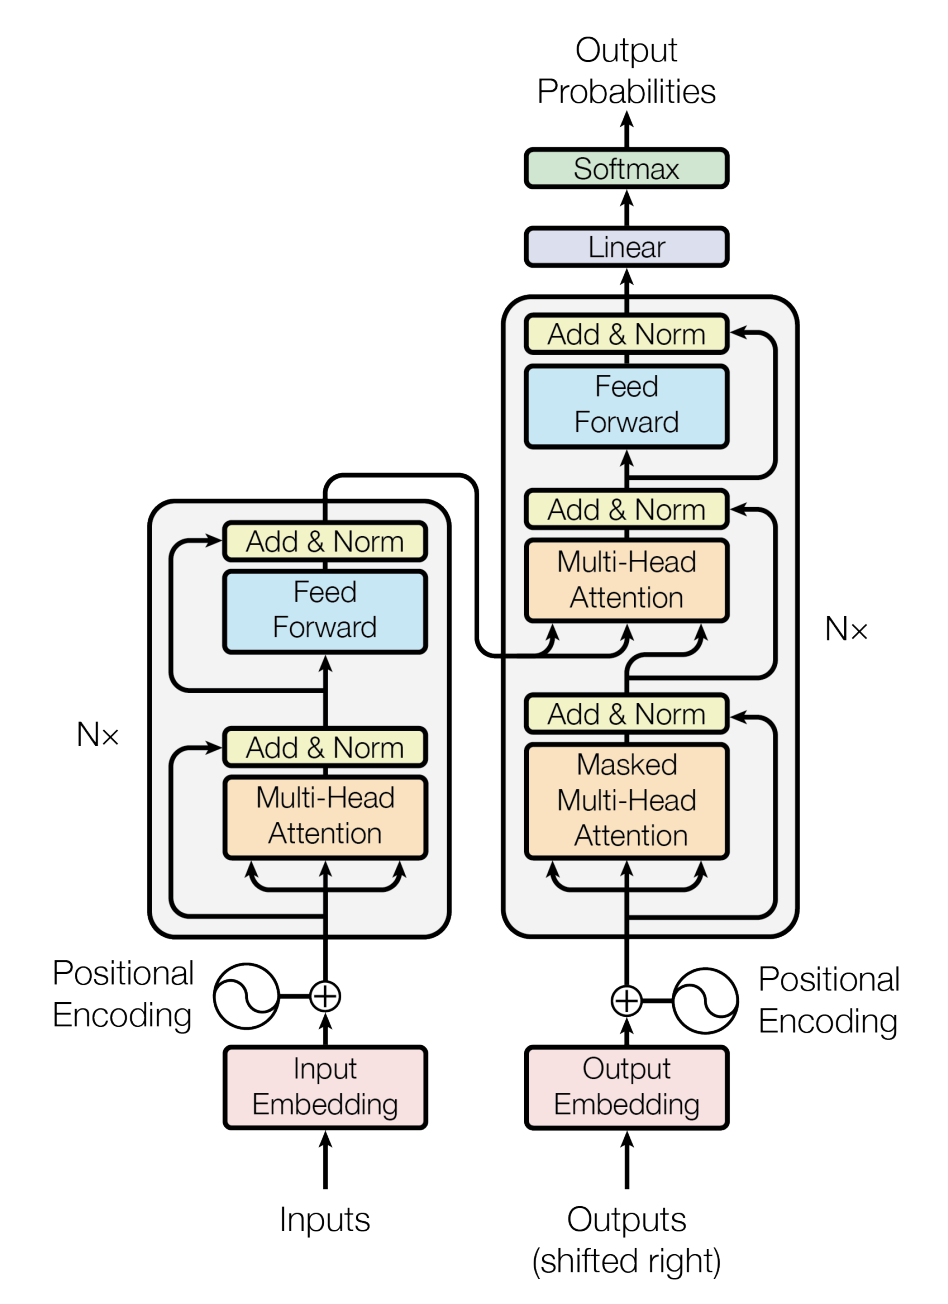
\includegraphics[width=0.4\textwidth]{figures/03_transformer_overview.png}
  \caption{Transformer model architecture. \cite{vaswani2017attention}}
  \label{fig:trans_arch}
\end{wrapfigure}
The input and output are first embedded into an $n$-dimensional space.
Since the network and the self-attention are permutation invariant,
the positional encoding is added to create a representation of the position of the word in the sentence.
The following modules consist mainly of Multi-Head Attention and Feed Forward layers. 
Encoder (Figure~\ref{fig:trans_arch}, left) and decoder (Figure~\ref{fig:trans_arch}, right)
are composed of those modules that can be stacked on top of each other $N\times$ times.

Self-attention is a sequence-to-sequence operation.
It takes a weighted average over all the input vectors using dot product.
Scaled Dot-Product Attention (Figure~\ref{fig:trans_attn}, left) can be described by the following equation:
\begin{equation} \label{eq:1}
Attention(Q,K,V) = softmax(\frac{QK^T}{\sqrt{d_k}})V
\end{equation}
where in the context of the translation problem,
$Q$ is a matrix of vector representation of one word in the sequence,
$K$ contains vector representations of all the words in the sequence and
$V$ contains again the vector representations of all the words in the sequence.
For the multi-head attention modules in the encoder and decoder,
$V$ consists of the same word sequence as $Q$.
However, for the attention module that is taken into account,
the encoder \underline{and} the decoder sequences, $V$, and $Q$ are different.
$Q$, $K$, and $V$ matrices are used to calculate the attention scores.
These scores measure how much attention needs
to be placed on words of the input sequence with respect to a word at a certain position.
The scaling factor $\sqrt{d_k}$ is applied to avoid large values that after 
applying softmax would lead to vanishing gradients.

While Scaled Dot-Product Attention focuses on the whole sentence, 
Multi-Head Attention approaches different segments of the words.
The word vectors are divided into a fixed number (number of heads) of parts,
and then within Multi-Head Attention (Figure~\ref{fig:trans_attn}, right) 
the attention mechanism is repeated multiple times on those separate parts with linear projections of $Q$, $K$, and $V$.
Since the Feed-Forward layer is expecting just one matrix, a vector for each word,
the outputs are linearly concatenated.
This allows the system to learn from different representations of $Q$, $K$, and $V$.

\begin{figure}[h] %h=here; t=top; b=bottom of the page
    \centering
    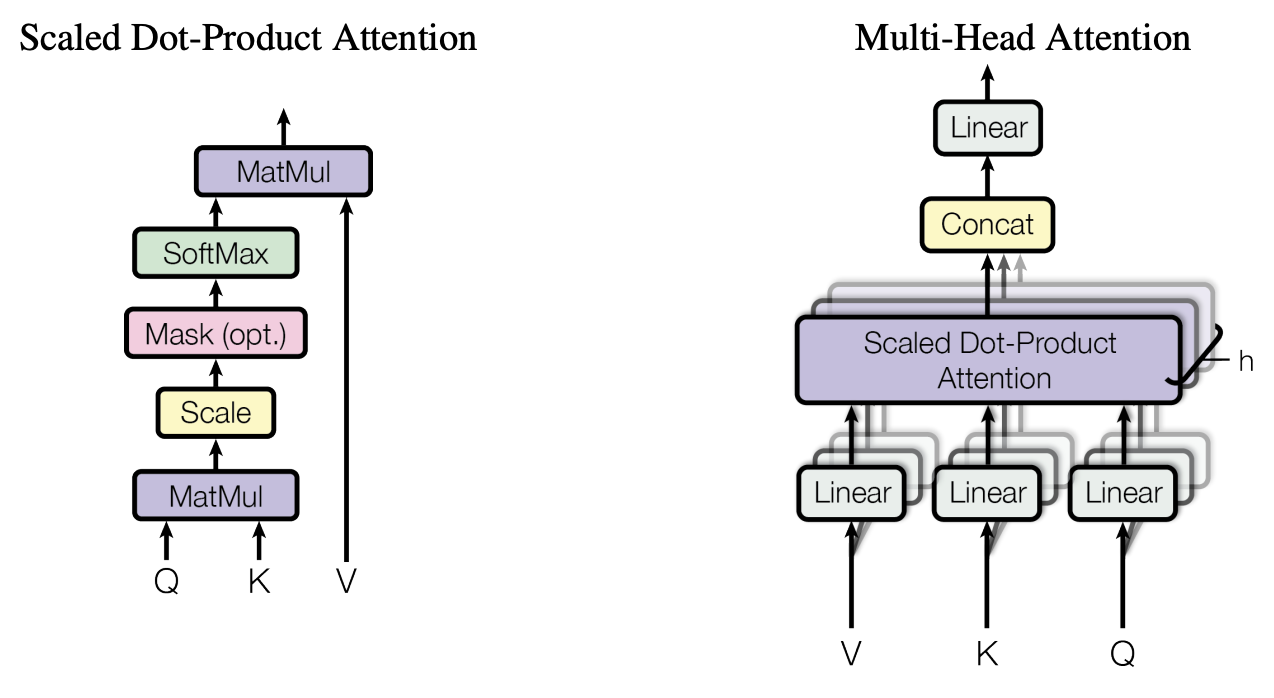
\includegraphics[width=0.7\textwidth]{figures/03_blocks_overview.png} %choose your uploaded image from folder "Images"
    \caption{Scaled Dot-Product Attention (left). Multi-Head Attention consists of several attention layers running in parallel (right). \cite{vaswani2017attention}} %figure caption
    \label{fig:trans_attn} %labelling for internal reference
\end{figure} 

To add element-wise non-linearity transformation of incoming vectors, 
the transformer includes feed-forward networks.
It processes the output from one attention layer so that it fits better for the next attention layer.
Each of the layers in the encoder and decoder contains a fully
connected feed-forward network, which is applied to each position separately and identically.
These feed-forward layers can be described as a separate, identical linear transformation of each element from the given sequence.

Naive application of the transformers approach into the image domain would require evaluation of relations between each pixel and every other pixel, which is obviously not scalable. The Visual transformer (ViT) \cite{dosovitskiy2020image} is the first work to prove that a pure Transformer can achieve state-of-the-art performance in image classification. ViT converts the input image into a 1D series by cutting it into patches and feeding it to a linear layer. It yields a patch embedding. Position embeddings are added to the image patch embeddings. Adding the learnable position embeddings to each patch allows the model to learn the structure of the image. The rest of the pipeline is a standard encoder and decoder blocks of the transformer.  The decoder learns to map patch-level encodings coming from the encoder to patch-level class scores. Next, these patch-level class scores are upsampled by bilinear interpolation to pixel-level scores.

\subsubsection{SegFormer}
SegFormer~\cite{xie2021segformer} is a positional-encoding-free transformer based semantic segmentation method. As depicted in Figure \ref{fig:segformer_over}, it consists of two main modules: a hierarchical Transformer encoder to generate high-resolution coarse features and low-resolution fine features, and a lightweight All-MLP decoder to fuse these multi-level features and produce the final semantic segmentation mask. 

\begin{figure}[h] %h=here; t=top; b=bottom of the page
    \centering
    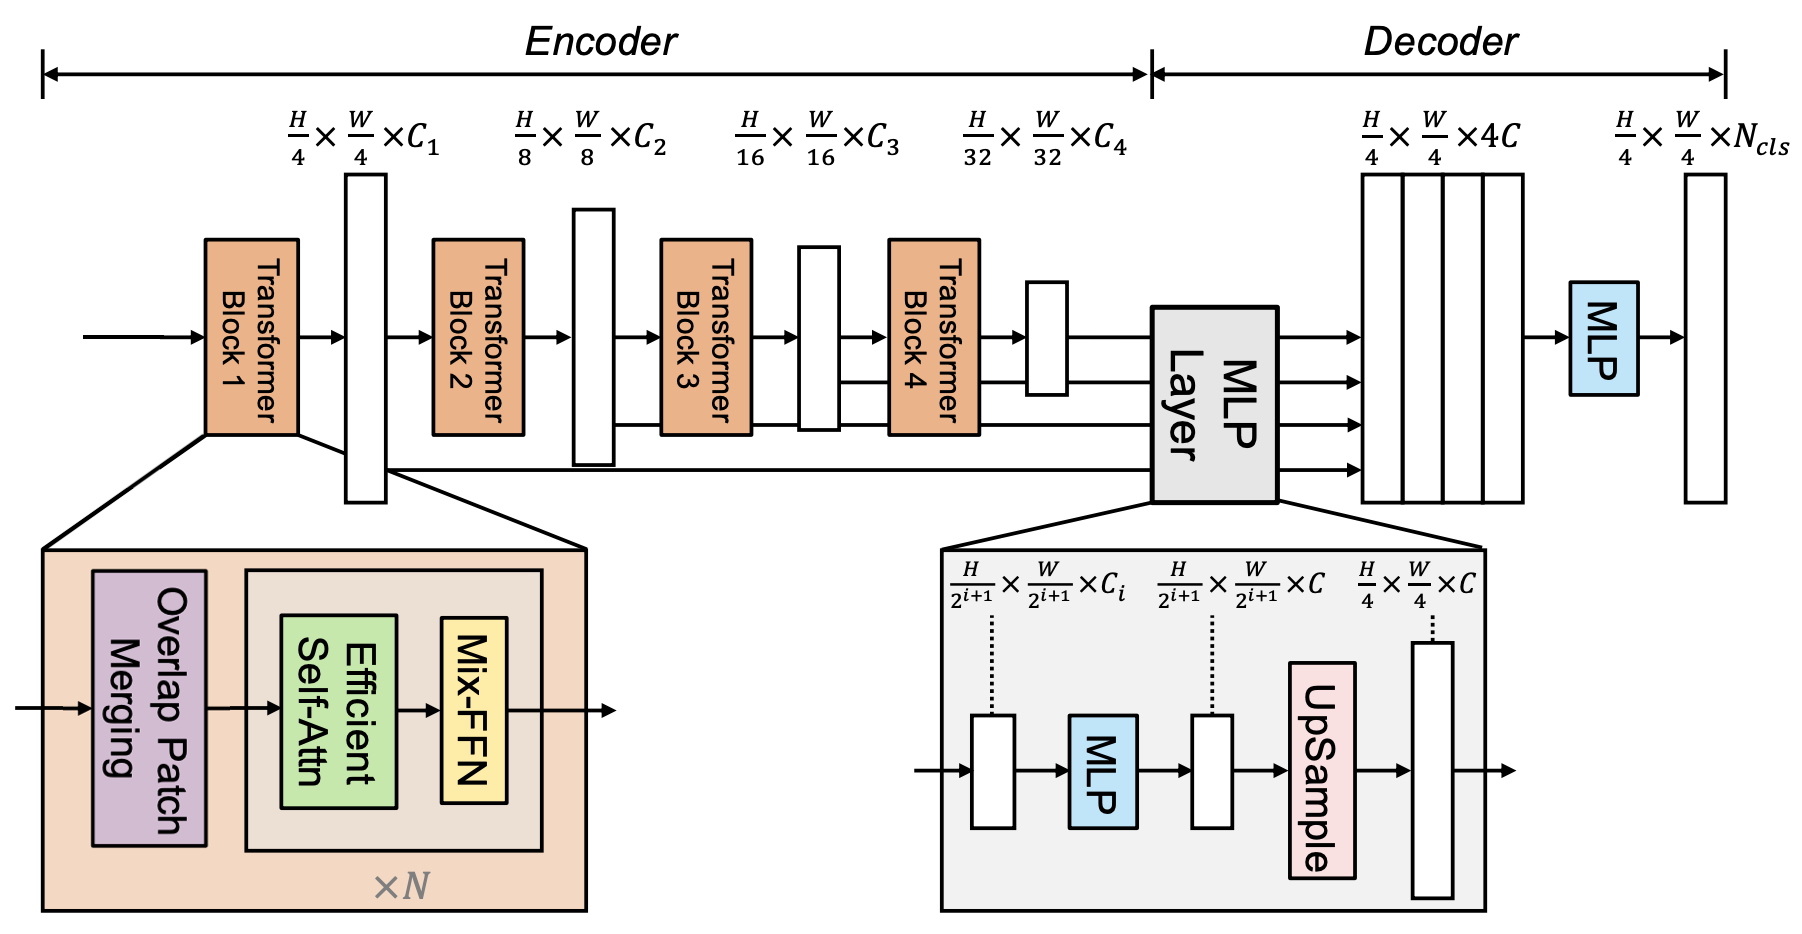
\includegraphics[height=60mm]{figures/03_segformer_overview.png} %choose your uploaded image from folder "Images"
    \caption{SegFormer consists of two main modules: A hierarchical Transformer encoder to extract coarse and fine features; and a lightweight All-MLP decoder to directly fuse these multi-level features and predict the semantic segmentation mask. “FFN” indicates feed-forward network. (modified image \cite{xie2021segformer} according to the official implementation)} %figure caption
    \label{fig:segformer_over} %labelling for internal reference
\end{figure} 

The $H\times W \times 3$ input image is forwarded to the hierarchical Transformer encoder to obtain multi-level features at $\frac{1}{4}, \frac{1}{8}, \frac{1}{16}, \frac{1}{32}$ resolution after passing through four transformer blocks.
Each transformer block consists of three modules: Overlap Patch Merging, and classical transformer building blocks: Self-Attention and Feed-forward network.

The standard transformer receives input as a 1D sequence (such as word embeddings in the previous chapter~\ref*{trans}).
To handle images, those need to be reshaped into a sequence of flattened 2D patches.
Overlapped Patch Merging produces features given an image and parameters: patch size $K$, stride between two adjacent patches $S$, and padding size $P$.
In the original paper~\cite{xie2021segformer} those are set to $K = 7$, $S = 4$ and $P = 3$.
Therefore the input is split into fixed-size patches, which then go through a linear projection.
The result is a hierarchical feature map $F_i$ with a
resolution $\frac{H}{2^{i+1}} \times \frac{W}{2^{i+1}} \times C_i$
where $i \in \{ 1,2,3,4\}$ and $C_{i+1}$ is larger than $C_i$.
By performing this with overlapped patches SegFormer aims to preserve the local continuity around those patches.

The main computation bottleneck of each transformer block in encoder is the self-attention layer. In SegFormer, before applying the self-attention according to the formula~\ref{eq:1}, the sequence $K$ is reduced by ratio $R$:
$$\hat{K} = Reshape(\frac{N}{R}, C\cdot R)(K)$$
$$K = Linear(C \cdot R, C)(\hat{K})$$
where $N = H \times W$, $Reshape(\frac{N}{R}, C \cdot R)(K)$ refers to reshaping $K$ to the the shape of $\frac{N}{R} \times (C \cdot R)$, and $Linear(C \cdot R, C)(\hat{K})$ refers to a linear layer taking a $(C \cdot R)$-dimensional tensor as input and generating a $C$-dimensional tensor as output. Therefore, the new $K$ has dimensions $\frac{N}{R} \times C$. 
In original experiments, $R$ was set to $[64, 16, 4, 1]$ from stage-1 to stage-4 and
resulted in a reduction of the complexity of the self-attention mechanism.

Mix-FFN (feed-forward network) can be formulated as:
$$x_{out} = MLP(GELU(Conv 3\times 3(MLP(x_{in})))) + x_{in}$$
where $x_{in}$ is the feature from the self-attention module. By using $3 \times 3$ convolution and zero padding in a feed-forward network SegFormer aims to leak pixel location information since it is a positional-encoding-free method.


The multi-level features are then passed to All-MLP decoder to predict the segmentation mask at $\frac{H}{4}\times \frac{W}{4}\times N_{cls}$ resolution, where $N_{cls}$ is the number of classes.
The proposed All-MLP decoder consists of four main steps. First, multi-level features from
the encoder go through an MLP layer to unify the channel dimension (\ref{eq:2}). Then, features are up-sampled to $\frac{1}{4}$th of the original image (\ref{eq:3}). Third, an MLP layer is adopted to fuse the concatenated features (\ref{eq:4}). Finally, another MLP layer takes the fused feature to predict the segmentation mask (\ref{eq:5}).
\begin{equation} \label{eq:2}
\hat{F_i} = MLP(C_i, C)(F_i), \forall i
\end{equation}
\begin{equation} \label{eq:3}
\hat{F_i} = Upsample(\frac{H}{4}\times \frac{W}{4})(\hat{F_i}), \forall i
\end{equation}
\begin{equation} \label{eq:4}
F = MLP(4C, C)(MLP(\hat{F_i})), \forall i
\end{equation}
\begin{equation} \label{eq:5}
M = MLP(C, N_{cls})(F)
\end{equation}
where $F_i$ is the the feature and $M$ is the final mask.

\subsection{TILs segmentation postprocessing}
As tissue segmentation, TILs detection was approached as a semantic
segmentation problem with detection bounding boxes transformed into
pseudo-segmentation masks (further details in Data section~\ref{section:data_segmentation}).
TILs segmentation results were first processed with non-maximum suppression
to extract local maxima, then obtain point annotation of each TIL, and compare
with ground truth annotations by finding a match with the Hungarian Algorithm.

\subsubsection{Non-maximum Suppression (NMS)}
Non-maximum Suppression is a class of algorithms to select
one entity out of many overlapping entities. In terms of
detection models, used to find the best-fitting bounding box out of all predicted
bounding boxes for the same object~\cite{bodla2017soft}.
Each proposal comes with a confidence score. One by one the bounding box with
the highest score is selected to keep and compared to all bounding boxes by calculating Intersection Over Union (IoU).
If a comparison scores the IoU higher than some defined threshold,
those bounding boxes out of the pool are eliminated.
The process is repeated by picking the highest confidence bounding box out of the
remaining pool of proposals until there are any.

In terms of TILs segmentation, there are no proposed bounding boxes and no scores.
Nonetheless, to obtain good centroids for each TILs prediction, the segmentation posteriors
need to be condensed to local maxima. The NMS application will in this case appropriately
filter the segmentation posteriors with a kappa threshold and the segmentation borders
refined to get a clear TIL region annotation with a suitable kernel size used for dilation.

\subsubsection{Hungarian algorithm}
To evaluate the match of predicted TILs and ground truth annotations,
it is not enough to compare the coordinates. Each TIL should be annotated
with a point annotation of one pixel, it is aimed to be placed in the center
but really placed in the center of a predicted TIL area, which is not perfect.
The goal is to find the pairs of coordinates that indicate the same TIL object.
Matching between the ground truth set and predictions can be solved as an assignment
problem with the Hungarian algorithm~\cite{kuhn1955hungarian}. It is a combinatorial
optimization algorithm that solves the problem in polynomial time complexity.
The distance matrix $n\times m$ between all annotated ($n$) versus predicted ($m$)
TILs is the cost matrix of each of the prediction coordinates to match any of the ground
truth coordinates. The goal is to assign the ground truth coordinates to the prediction
coordinates to minimize the total distance. The algorithm can be introduced as step-by-step instruction:
\begin{itemize}
  \itemsep0em 
  \item Step 1: For each row, subtract the smallest element of the row from each of its elements.
  \item Step 2: For each column, subtract the smallest element of the column from each of its elements.
  \item Step 3: Cover all zeros with a minimum number of lines
  \item[] In the resulting matrix cover all zeros using a minimum number of horizontal and vertical lines. 
  If there are $n$ lines, Step 5.
  \item Step 4: Find the smallest element that is not covered by a line in Step 3.
  Subtract it from all uncovered elements, and add it to all elements that are covered twice. Step 3.
  \item Step 5: Assignment pairs are indicated by the positions of the zeros in the cost matrix. 
\end{itemize}
As a result, the assignment pairs include the matching of ground truth TILs coordinates to the
prediction coordinates that minimize the total distance. If desired, the pairs can be filtered
by minimal allowed distance. This work uses the \verb+scipy.optimize.linear_sum_assignment+
implementation of the Hungarian algorithm.

\section{Survival Analysis}
The overall survival (OS) is the primary endpoint for prognostic analysis in this thesis,
hence time to the event (death) is of interest. 
Survival data are generally described and modeled in terms of two related probabilities, namely survival and hazard.~\cite{clark2003survival}
This thesis focuses on non-parametric models to avoid making any additional assumptions about the distributions.
Throughout the analysis, the python library \verb+lifelines+~\cite{davidson2019lifelines} was used.
The survival probability $S(t)$ is the probability that an individual survives from the time origin (in our case diagnosis of breast cancer) to a specified future time $t$.
It can be denoted as: $$S(t) = Pr(T>t) = 1-F(t) = \int_t^\infty f(x) dx = \textrm{ Probability of surviving past time } t $$
where $T$ is a random variable that indicates the time until the event of interest (death). $F(t)$ and $f(t)$ are the cumulative distribution function
and probability density function of $T$. 
The hazard is the probability that an individual who is under observation at a time $t$ has an event at that time:
$$h(t) = lim_{\delta t \rightarrow 0}\frac{Pr(t \leq T \leq t + \delta t | T > t)}{\delta t} = \frac{f(t)}{1-F(t)}$$
In contrast to the survival function, which focuses on not having an event, the hazard function focuses on the event occurring. 
So if hazard probability describes the intensity of death~\cite{STAT_425} at the
time $t$ given that the individual has already survived past time $t$, then
the cumulative hazard is the cumulative amount of hazard up to time $t$.
The cumulative hazard $H(t)$, defined as the integral of the hazard,
can be calculated using the survival probability with help of the Laplace transform:
$$ H(t) = \int_0^t h(x) dx = \int_0^t \frac{f(x)}{1-F(x)} dx = - ln(1 - F(t)) = - \log (S(t)) $$
The cumulative hazard can be interpreted as the number of events that would be expected for each individual by time $t$ if the event was a repeatable process.~\cite{clark2003survival}

\subsection{Kaplan–Meier estimator}
The survival probability can be estimated nonparametrically from observed survival times,
both censored and uncensored, using the Kaplan–Meier method.
The estimated probability of surviving past time $t$ is calculated as:
$$\hat{S}(t) = \prod_{i; t_i \leq t} (1-\frac{d_i}{n_i})$$
where $n_i$ is the number of patients alive before $t_i$ (and not censored) and $d_i$ is the number of observed events at $t_i$. $t_0=0$ and $S(0)=1$.
The estimated probability is a step function that changes value only at the time of an event.
To characterize the survival in a homogeneous group often the empirical survival function is visualized with Kaplan–Meier plot.

\subsection{Cox model}
Additionally to the event time, there is often access to other covariates
of individuals (e.g. age, gender, BMI, etc.). Often the goal is to understand how the covariates affect
the survival function of the event.~\cite{STAT_425}
Let $C$ denote those covariates. The conditional survival function can be formulated
as followed:
$$S(t|c) = Pr(T>t|C=c) = \textrm{ Probability of surviving past time } t \textrm{ given } c$$
Hence, the conditional hazard function and conditional cumulative hazard are:
$$ H(t|c) = - \log (S(t|c)) \textrm{, hence } h(t|c) = -\frac{\partial \log S(t|c)}{\partial t}$$
The Cox proportional hazard model models the hazard function $h(t|C=c)$ as:
$$h(t|C=c) = h_0(t) \exp(c^T \beta)$$
where $\beta$ is the vector of coefficients for each of the covariates and $h_0(t)$ is the baseline hazard
function. The hazard ratio, or \textbf{\textit{risk}}, is the exponential of $\beta_i$ value $\eta_i = \exp(\beta _{i})$ and the baseline hazard describes how the risk of event per time unit changes over time at baseline levels of covariates. The Cox model assumes that the covariates have a linear multiplication effect on the
hazard function and the effect stays the same over time. 
$$\frac{h(t|c_i)}{h(t|c_j)} = \frac{h_0(t) \exp(c_i^T \beta)}{h_0(t) \exp(c_j^T \beta)} = \frac{\exp(c_i^T \beta)}{\exp(c_j^T \beta)} =  \exp((c_i - c_j)^T \beta)$$
The ratio of the hazard function between two individuals with different covariates $c_i$ and
$c_j$ is a constant over time since $h_{0}(t)$  was canceled out. Hence the name, proportional hazard model. The conditional hazard function is:
$$H(t|c) = \exp(c^T \beta) \int_0^t h_0(s) ds = \exp(c^T \beta)H_0(t)$$
It yields a conditional survival function:
$$S(t|c) = \exp (-H(t|c)) = \exp(-\exp(c^T \beta)H_0(t)) = \exp(-H_0(t))^{\exp(c^T \beta)} = S_0(t)^{\exp(c^T \beta)}$$
Estimation of the parameter $\beta$ is often done by maximizing the partial likelihood function $\hat{\beta}_n = argmax_\beta \hat{L}_n(\beta) $, where:
$$ \hat{L}(\beta) = \prod_{i=1}^n \frac{h(T_i|C_i)}{\sum_{j: T_j \geq T_i} h(T_j|C_j)} = \prod_{i=1}^n \frac{\exp(C_i^T \beta)}{\sum_{j: T_j \geq T_i} \exp(C_j^T \beta)}$$
A positive sign of $\beta_i$ indicates a higher risk of an event, hence the probability for the event for that particular subject is higher. Likewise for a negative signed $\beta_i$, lower risk, and lower probability. The actual value of $\beta_i$ plays a role as well. Values less than one will reduce the hazard and values greater than one, increase it.

A model's accuracy can be quantified based on concordance.~\cite{therneau20201} 
It is a measure of the rank correlation between predicted risks and observed time points. 
It is defined as the ratio of correctly ordered (concordant) patient pairs to all concordant and discordant patient pairs.
Let $i, j$ be a patient pair. If a model predicts a higher risk for the first patient ($\eta_i > \eta_j$), for it to be a concordant pair first patient should have a shorter survival time in comparison with the other patient ($ T_i < T_j$) and similarly if lower risk then longer survival time, $\eta_i < \eta_j \And T_i > T_j$.
If both patients are censored the pair is discarded.
If only one patient is censored, the pair is not discarded only if the other patient experienced the event before the censoring time. By construction, concordance must be between $0$ and $1$, with $1$
representing the perfect agreement between model and
observation and $0.5$ representing random guesses.

Additionally, to estimate the goodness-of-fit the p-value is determined. The Wald test is typically used to evaluate the significance of a variable in the model estimated with the maximum likelihood function. The null hypothesis is that the model does not fit the data well. The Wald statistic tests, whether $\beta_i$ coefficient is statistically significantly different from $0$ and is defined as:
$$ W=\frac{(\hat{\beta}_n-\beta_0)^{2}}{var(\hat{\beta}_n)}$$
If the true coefficient was $\beta_0$, then the sampling distribution of
the Wald test statistic should be approximate $\mathcal{N} (0, 1)$. 
The p-value gives the probability of observing a test statistic as extreme as the one observed if the sampling distribution was $\mathcal{N} (0, 1)$. If the p-value is small, the observed test statistic is very
unlikely under the null hypothesis. And the significance level of $0.05$ indicates that there is a $5\%$ risk of being wrong by concluding that the model fits the data well when it doesn't.